\let\negmedspace\undefined
\let\negthickspace\undefined
\documentclass[journal]{IEEEtran}
\usepackage[a5paper, margin=10mm, onecolumn]{geometry}
%\usepackage{lmodern} % Ensure lmodern is loaded for pdflatex
\usepackage{tfrupee} % Include tfrupee package
\setlength{\headheight}{1cm} % Set the height of the header box
\setlength{\headsep}{0mm}     % Set the distance between the header box and the top of the text
\usepackage{gvv-book}
\usepackage{gvv}
\usepackage{cite}
\usepackage{amsmath,amssymb,amsfonts,amsthm}
\usepackage{algorithmic}
\usepackage{graphicx}
\usepackage{textcomp}
\usepackage{xcolor}
\usepackage{txfonts}
\usepackage{listings}
\usepackage{enumitem}
\usepackage{mathtools}
\usepackage{gensymb}
\usepackage{comment}
\usepackage[breaklinks=true]{hyperref}
\usepackage{tkz-euclide} 
\usepackage{listings}
% \usepackage{gvv}                                        
\def\inputGnumericTable{}                                 
\usepackage[latin1]{inputenc}                                
\usepackage{color}                                            
\usepackage{array}                                            
\usepackage{longtable}                                       
\usepackage{calc}                                             
\usepackage{multirow}                                         
\usepackage{hhline}                                           
\usepackage{ifthen}                                           
\usepackage{lscape}
\usepackage{circuitikz}
\tikzstyle{block} = [rectangle, draw, fill=blue!20, 
    text width=4em, text centered, rounded corners, minimum height=3em]
\tikzstyle{sum} = [draw, fill=blue!10, circle, minimum size=1cm, node distance=1.5cm]
\tikzstyle{input} = [coordinate]
\tikzstyle{output} = [coordinate]
\begin{document}
\bibliographystyle{IEEEtran}
\vspace{3cm}
\title{9.8.19}
\author{AI25BTECH11017-BALU}
 \maketitle
% \newpage
% \bigskip
{\let\newpage\relax\maketitle}
\renewcommand{\thefigure}{\theenumi}
\renewcommand{\thetable}{\theenumi}
\setlength{\intextsep}{10pt} % Space between text and floats
\numberwithin{equation}{enumi}
\numberwithin{figure}{enumi}
\renewcommand{\thetable}{\theenumi}
\textbf{Question}:\\
\begin{enumerate}
    \item Two circles $x^{2}+y^{2}=6$ and $x^{2}+y^{2}-6x+8=0$ are given. 
    Then the equation of the circle through their points of intersection 
    and the point $(1,1)$ is (1980)
    \begin{enumerate}[label=(\alph*)]
        \item $x^{2}+y^{2}-6x+4=0$
        \item $x^{2}+y^{2}-3x+1=0$
        \item $x^{2}+y^{2}-4y+2=0$
        \item none of these
    \end{enumerate}
\end{enumerate}
\solution \\
Let us solve the given equation theoretically and then verify the solution computationally \\
According to the question, \\
equation circles are
\begin{align}
\vec{X}^T\vec{X}-6=0\\
\vec{X}^T\vec{X}+2\myvec{-3&&0}\vec{X}+8=0
\end{align}
substute 1.1 in 1.2
\begin{align}
  \myvec{-3&&0}\vec{X}=-7\\
  x=\frac{7}{3}
\end{align}
substute 1.4 in 1.1
\begin{align}
   y=\frac{\sqrt{5}}{3},\frac{-\sqrt{5}}{3}
\end{align}
let equation of requried circle is
\begin{align}
  \vec{X}^T\vec{X}+2\vec{u}^T\vec{X}+f=0\\
  \vec{u}^T\myvec{1\\1}=\frac{-f}{2}-1\\
  \vec{u}^T\myvec{\frac{7}{3}\\\frac{\sqrt{5}}{3}}=\frac{-f}{2}-3\\
  \vec{u}^T\myvec{\frac{7}{3}\\\frac{-\sqrt{5}}{3}}=\frac{-f}{2}-3
\end{align}
\begin{align}
    \myvec{1&&1\\\frac{7}{3}&&\frac{\sqrt{5}}{3}\\\frac{7}{3}&&\frac{-\sqrt{5}}{3}}\vec{X}=\myvec{\frac{-f}{2}-1\\\frac{-f}{2}-3\\\frac{-f}{2}-3}
\end{align}
\begin{align}
   \operatorname{rank}\myvec{1&&1&&\frac{-f}{2}-1\\\frac{7}{3}&&\frac{\sqrt{5}}{3}&&\frac{-f}{2}-3\\\frac{7}{3}&&\frac{-\sqrt{5}}{3}&&\frac{-f}{2}-3}=2\\
   f=1\\
   \vec{u}=\myvec{\frac{-3}{2}\\0}
\end{align}
the reqiured circle equation is
\begin{align}
    x^2+y^2-3x+1=0
\end{align}
\begin{figure}[h!]
    \centering
    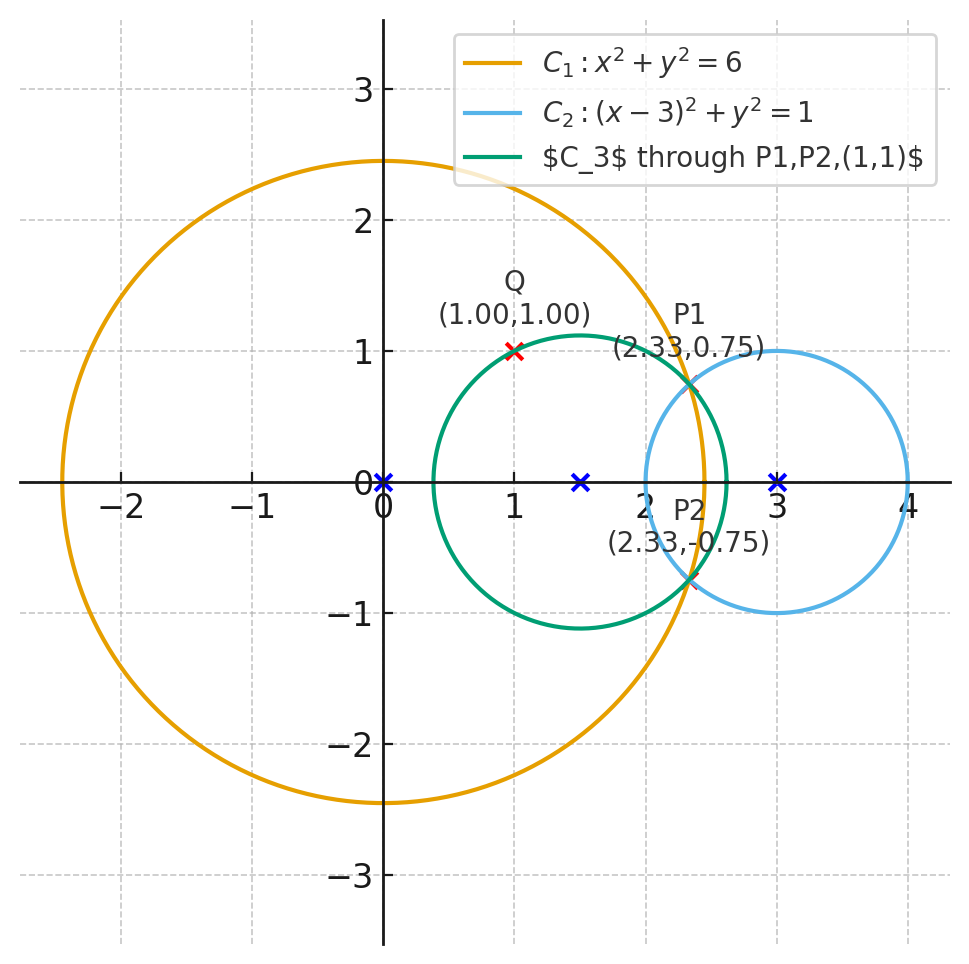
\includegraphics[width=0.5\linewidth]{figs/circles.png}
    \caption{}
    \label{fig:placeholder}
\end{figure}
\end{document}